	Nous allons, dans cette partie, décrire les travaux concernant la mise en place d'une procédure complète permettant de gérer et réaliser des tests fonctionnels de manière automatique et fournissant des rapports complets pouvant être remis au client.

\subsection{Enjeux et spécifications}
		Comme nous l'avons vu précédemment, les services de nos API rest sont destinés à être consommés par PBI, en charge du développement de la partie frontend de l'application mobile. Ainsi, nous étions souvent en contact avec ces derniers afin de prendre connaissance des différentes anomalies liées à nos services et de pouvoir répondre à l'évolution de leur besoins. Après correction de celles-ci, il était fréquent que nous soyons amenés à livrer la nouvelle version des services. Ces livraisons permettaient à PBI de pouvoir continuer le développement de l'application dans les meilleures conditions possibles. Elles s'effectuaient sur deux environnements différents à savoir \textit{homo3} et \textit{rgb} comme il est possible de l'observer sur la figure \ref{environnement}. \\
	
	L'environnement homo3 est un serveur d'homologation sur lequel était effectué les recettes avec le client. Celui-ci permet de réaliser des tests afin de s'assurer que le produit est conforme aux spécifications. L'environnement rgb est un serveur de pré-production dont la structure, contrairement à homo3, est identique à celui de la production. Ce serveur permet de réaliser un béta test du produit ainsi que des tests de charge par le client dans des conditions réelles afin de déceler les derniers bug potentiels avant la mise en production. De son côté, PBI, possède la même structure avec un serveur de recette nommé \textit{ST} et un environnement de pré-production nommé \textit{ET} connectés à nos environnements. Ainsi, nous partagions les mêmes données pour réaliser nos tests (identifiants utilisateur, comptes bancaires, portefeuilles, positions, transactions...) Concernant les services EFS nous étions toujours sur leur production ou sur des mocks (objets simulés reproduisant le comportement d’objets réels) en attendant la mise en production des services demandés.\\
	
	Cependant, avant de procéder à la livraison des services sur ces environnements, il est nécessaire d'effectuer une batterie de tests fonctionnels permettant de vérifier que le comportement des API est conforme aux spécifications. Ces tests sont essentiels à la satisfaction client et permettent de gagner un temps précieux en évitant d'attendre les retours avant d'identifier les possibles anomalies. Nous réalisons beaucoup d'évolutions et de corrections de bugs qui parfois impliquent des effets non désirés qui peuvent être décelés par de tels tests. Néanmoins, dans notre cas, peu de ces tests avaient été mis en place et il n'existait aucune procédure à suivre. Les cas de tests était rédiger sous Word et le résultat de leur exécution était consigné dans des fichiers excel, peu lisibles, contenant peu d'informations et difficilement traçables. De cette manière, il est difficile de normaliser l'écriture des tests et la création d'un rapport est chronophage (créer les formules excel, etc...) pour un résultat qui ne sera pas exhaustif. En outre, il est impossible d'avoir une vue d'ensemble sur l'évolution des tests au cours du temps et est compliqué de suivre l'état d'une spécification particulière à différentes dates données. Par ailleurs, le client lui-même a souhaité un autre format plus rigoureux permettant de vérifier le comportement des services dans leur intégralités et de pallier aux inconvénients que nous avons cité. \\	
	
\begin{figure}[h!]
	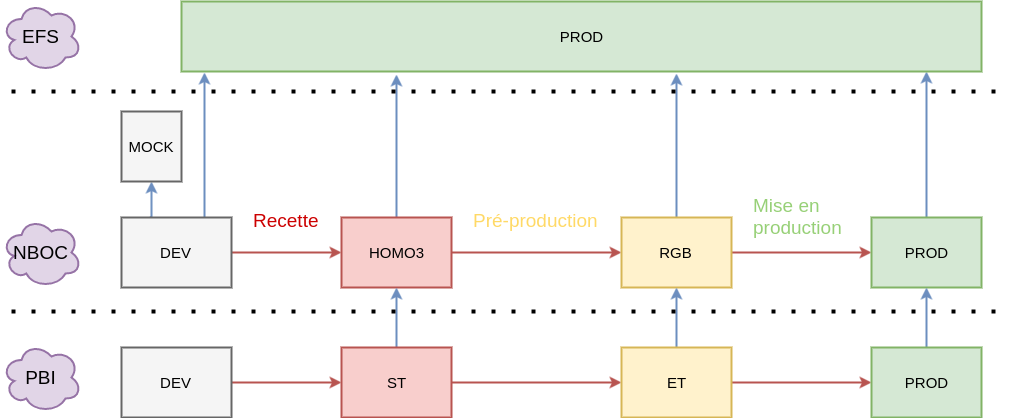
\includegraphics[scale=0.5]{images/travailNeuflizeOBC/testsFonc/environnement.png}
	\center
	\caption{Environnements}
	\label{environnement}
\end{figure}

	Ainsi, j'ai été chargé de mettre en place une procédure pouvant répondre à ce besoin. Cette dernière devait :	
	\begin{itemize}
		\item définir les cas de tests
		\item fournir des rapports d'exécution de tests détaillés
		\item nécessiter peu de développement, il était en effet inutile de réinventer la roue
		\item être gratuite
		\item être accessible à tout moment à n'importe quel membre de l'équipe de développement qui pourrait être amené à effectuer une livraison \\
	\end{itemize}
	\label{testsFonc_01}

\subsection{TestLink : Un gestionnaire de tests}
		Dans le but de répondre aux besoins explicités précedemment, j'ai décidé d'avoir recours à un gestionnaire de tests sous forme d'une application web. En effet, celle-ci pourrait être mise en place sur un seveur interne et rendue disponible pour toute l'équipe, favorisant ainsi le partage d'information et permettant de centraliser toutes les données concernant la réalisation des tests fonctionnels, assurant ainsi un versionning cohérent. De plus, cela répond à la problématique de mise en place rapide et de maintenabilité efficace (pas de mise à jour à gérer sur tous les postes, etc...). \\
	
	Après avoir mené plusieurs recherches, j'ai pu constater qu'il existait différents gestionnaires open-source concurrents sur le marché répondant à nos exigences : \textit{Salomé TMF}, \textit{TestLink} ou encore \textit{Squash TM}. En effet, ces derniers nous offrent tous la possibilité de créer des tests, de les lier aux exigences client ou encore de créer des campagnes de tests puis d'exporter les résultats sous forme de rapport détaillé. Ces outils proposant des fonctionnalités très proches, j'ai décidé d'en choisir un disposant d'une grande flexibilité ainsi que d'une communauté active afin de pouvoir faciliter l'adaptation à nos cas de tests. En effet, les gestionnaires génèrent des rapports regroupant des informations telles que la description des tests, leur temps d'exécution ou leur status. Cependant, dans notre cas, nous souhaitions pouvoir inclure pour chacun des tests des informations supplémentaires telles que le nom du service auquel appartient la fonctionnalité testée, l'identifiant de l'utilisateur utilisé pour le test, le numéro de compte bancaire utilisé et de manière générale, tous les paramètres utilisés pour réaliser la reqûetes testées. PBI partageant les mêmes données que nous sur les environnements d'homologatoin et de pré-production, il leur était alors possible de vérifier de leur côté que les tests passent effectivement. De plus, lorsqu'ils remarquaient une anomalie, ils pouvaient nous transmettre les paramètres qu'ils avaient utilisé afin que nous puissions reproduire celle-ci chez nous. \\
	
	Ainsi, j'ai décidé d'utiliser l'outil \textit{TestLink} dont la communauté avait mis à disposition de tous des templates permettant de modifier le code source afin de customiser la génération des rapports de tests. Celui-ci est une application web développée en PHP et utilisant le système de gestion de base de données MySQL. Il permet de centraliser toute la gestion des tests fonctionnels du projet en les organisant par le biais des structures présentées dans le tableau \ref{structuresTestlink}.

\begin{table}[h!]
	\center
	\begin{tabular}{| c | c |}
     \hline
     Cas de test & Test fonctionnel définissant un scénario spécifique \\ \hline
     Suite de tests & Collection de cas de test validant une même fonctionnalité \\ \hline
     Plan de tests & Collection de suite de tests contenant toutes les informations \\  & telles que la portée, les étapes, la version etc...\\ & Un plan est exécuté pour un build particulier \\ \hline
     Build & Une release spécifique des APIs testées \\
     \hline
	\end{tabular}
	\caption{Structures fournies par TestLink}
	\label{structuresTestlink}
\end{table}

Cet outil présente de nombreux avantages qui m'ont conforté dans mon choix :
\begin{itemize}
	\item Campagnes de tests versionnées dont l'historique est enregistré en base de données.
	\item Export et import de cas de test et de leur résultats
	\item Connection avec \textit{Mantis}, un tracker de bug utilisé dans notre projet
	\item Gestion de rôles sur les tests (qui effectues le test, qui valide etc...)
	\item Rapport complet dans différents formats
	\item Accessible à toute l'équipe n'importe quand 
	\item Simplicité d'utilisation et de mise en place \\
\end{itemize}

	Ensuite, avant de procéder à la création des cas de test sur TestLink, j'ai commencé par définir la structure du futur plan de test qui serait exécuté avant chaque livraison. Ainsi, j'ai décidé de séparer l'ensemble des tests en deux grandes familles : ceux concernant les fonctionnalités de consultation et ceux concernant les fonctionnalités de transaction, ce qui m'amena à la création de deux suites de tests. Après cela, j'ai créé autant de suites de tests qu'il y avait de fonctionnalités décrites dans l'annexe \ref{a2}. Il est possible d'observer sur la figure \ref{testlink} l'organisation d'un plan de test type. Afin de garder le même formalisme tout le long de la réalisation des plans de tests et pour assurer une certaine cohérence, j'ai décidé de mettre en place plusieurs conventions définissant une stratégie de test :
	
	\subsubsection*{Cas de test}
	Les cas de tests doivent avoir un nom de la forme [id]-[titre] où
	\begin{itemize}
		\item id désigne un ID unique permettant de les identifier rapidement et de faciliter leur organisation. Celui-ci est \textit{NOBC-API-XX}, où XX représente le numéro du test. 
		\item titre désigne de manière clair et concise l'objectif du test
	\end{itemize}		
	De plus, chaque cas de test possède en attribut un numéro de version de la forme \textit{vX} où X est incrémenter de 1 chaque fois que le cas de test est modifié.
	
	\subsubsection*{Plan de test}
	Les plans de tests doivent avoir un nom de la forme [scope]-[environnement]-[version] où
	\begin{itemize}
		\item scope désigne la portée du plan de test : "complete" pour tous les tests, "transaction service" pour les tests du service de transaction, "transaction overview" pour les tests de la fonctionnalité transaction overview etc...
		\item environnement désigne le serveur sur lequel sont effectués les tests : homo3 ou rgb
		\item version est de la forme vX.Y.Z où
			\begin{itemize}
				\item X est incrémenté de 1 lorsqu'un nouveau cas de test est ajouté ou supprimé du plan
				\item Y est incrémenté de 1 lorsqu'un cas de test existant du plan a été modifié
				\item Z est incrémenté de 1 à chaque exécution du plan
			\end{itemize}
	\end{itemize}
	
	\subsubsection*{Build}
	Les builds doivent avoir un nom de la forme : [version] où
	\begin{itemize}
		\item version désigne la version de l'API microservices testée \\
	\end{itemize}

	La stratégie de test étant définie, il fallait maintenant déterminer quelles informations devaient être transmises au sein des rapports de tests. Les gestionnaires de tests proposent de remplir des formulaires afin consigner le résultat des tests une fois ceux-ci effectués, ce qui servira par la suite à générer un rapport. Cependant, ces derniers sont plutôt génériques et ne permettent pas de renseigner des données spécifiques à un projet particulier. Comme nous l'avons dit plus haut, nous souhaitions être en mesure de passer des paramètres supplémentaires afin de faciliter nos échanges avec PBI, comme : \\
	
	\begin{itemize}
		\item url et paramètres utilisés pour la requête
		\item service testé
		\item identifiants utilisés
	\end{itemize}
	
	\begin{figure}[h!]
	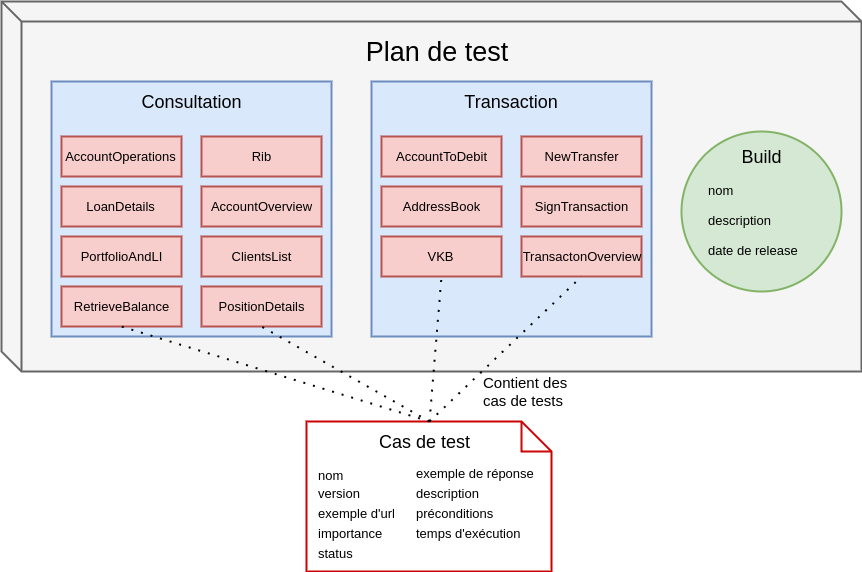
\includegraphics[scale=0.5]{images/travailNeuflizeOBC/architecture/testlink.png}
	\centering
	\caption{Configuration d'un plan de test type}
	\label{testlink}
\end{figure}
	
	Ainsi, j'ai décidé de modifier le code source de TestLink afin de rajouter les champs dont nous avions besoin aux formulaires de tests. J'ai réalisé cette modification en deux étapes dont la première consistait à ajouter les champs aux formulaires puis à gérer la partie front en PHP. La seconde concernait la récupération des données et leur sauvegarde en base de données, ce qui a impliqué la création de nouvelles requêtes SQL. Une fois les champs mis en place, j'ai créé un cas de test puis générer un premier rapport au format PDF en guide de POC (proof of concept). Celui-ci ayant été jugé satisfaisant, j'ai dû étudier l'ensemble des spécifications du projet concernant chacun des services mis en place afin de procéder à l'écriture de tous les cas de tests. Cela m'a permis de mieux comprendre le besoin du client, d'avoir une bien meilleure vision sur le projet dans sa globalité en m'apportant des informations sur l'utilité de chaque service et de pouvoir me former sur le projet en restant productif.
	
	Ces cas de tests permettaient de vérifier que les réponses des requêtes émises vers l'API microservices étaient en accord avec les attentes de PBI. Par exemple, les réponses étant au format JSON, ils permettaient la vérification de la présence de tous les champs obligatoires, la cohérence des valeurs des champs (\hl{TODO exemple a prendre dans la spec}) ou encore la vérification de la cohérence des données de notre backend avec celles de l'application web.
	\label{testsFonc_02}
	
\subsection{Rapports de tests obtenus}
		Une fois tous les cas de tests rédigés, j'ai procédé à la réalisation d'une campagne de tests complète aboutissant à la génération d'un rapport. Afin de procéder à cela, pour chacun des tests j'ai utilisé l'outil \textit{Postman} qui est une plateforme proposant une interface graphique facilitant la construction de requêtes. Cet outil est conçu pour faciliter le développement des APIs en permettant de les intéroger de manière très rapide et simple sans avoir à développer un client pour les consommer. Dans l'optique de mettre à profit les tests effectués, nous avons connecté TestLink à Mantis, une application web permettant d'assurer le suivi des anomalies dans laquelle il est possible d'ouvrir des tickets concernant des bugs qui seront alors pris en charge par les développeurs jusqu'à leur clôture. Ainsi, lorsqu'un test échouait il était possible, d'un simple clique sur TestLink, de générer automatiquement un ticket sur Mantis avec toutes les informations rajoutées précédemment. Les développeurs avaient donc toutes les données (url, service etc...) pour reproduire l'anomalie en locale et la corriger. \\
	
	TestLink permet de personnaliser la génération des rapports de tests après l'exécution d'un plan complet. De plus, il est possible de générer le rapport dans différents formats. Nous avons donc décidé que chaque livraison comporterait un rapport complet contenant toutes les informations au format PDF. Cependant celui-ci pouvant être très conséquent, nous avons choisi de l'accompagner d'un rapport léger généré au format excel ne contenant que le nom des tests et leur statut (succès, echec, bloqué) avec un code couleur permettant a PBI de rapidement repérer les tests en échec et leur nombre. Ces derniers ont déclaré être très satisfait des nouveaux rapports fournis, c'est pourquoi il a été décidé que l'exécution des tests fonctionnels sur la plateforme TestLink serrait obligatoire avant chaque livraison. En attendant l'attribution d'un serveur pour héberger le gestionnaire de test, celui-ci a été mis en place sur le serveur personnel d'un des architecte du projet afin de le rendre accessible à toute l'équipe. \\
	
	La réalisation de ces tests et leur exécution m'a permis de relever certains écarts entre le produit réalisé et les spécifications. Par exemple \hl{TODO : exemple d'ecarts loanDetails}. C'est pourquoi, après avoir centralisé tous les écarts que j'avais relevé, j'ai organisé une réunion avec mon chef de projet ainsi que certains développeurs dans le but de déterminer lesquels pourraient être corriger et lesquels ne le pourraient pas, nécessitant de prendre contact avec le client afin de clarifier la situation. Au terme de cette réunion, j'ai pu créer une nouvelle version des spécifications afin de les mettre à jour puis j'ai fait part de ces modifications à PBI à travers des mails rédigés en anglais. Ensuite, la mise en place de ces outils a permi à l'équipe de pouvoir effectuer les livraisons dans de meilleurs conditions puisque les anomalies pouvaient être détectées avant d'attendre les retours du client. De plus, tous les tests étaient centralisés, organisés et pouvaient être exécutés en parallèle par différentes personnes ce qui permettait un gain de temps à la fois sur l'exécution des tests mais aussi sur leur gestion (archivage, formalisme, perte de documents etc...). \\
	
	Néanmoins, afin d'exécuter les tests, les développeurs utilsaient Postman pour construire et envoyer les requêtes. Si cet outil est extrèmement utile pour développer un nouveau service ou tester un nouveau endpoint lors du développement, il n'est pas conçu pour exécuter un grand nombre de requête les unes après les autres à des fins de tests. En effet, comme nous l'avons expliqué dans la partie \ref{axway} les requêtes doivent posséder un token d'authentification dans leur header pour espérer passer la gateway et atteindre la couche microservices. Or, pour cela, il est nécessaire d'envoyer, toujours avec Postman, une requête de génération de ce token à l'API gateway. Après cela, il faut se connecter sur l'interface web fourni par Axway, retrouver la requête ainsi que sa réponse et copier le token. Cependant, pour accéder à cette interface il faut d'abord être en mesure d'accéder à l'environnement testé, Homo3 ou RGB, qui, rappelons le, n'ont pas les mêmes instances de l'API Gateway et ne sont pas accessibles de l'extérieur. Pour cela, il faut se connecter en RDP sur TSE puis ensuite utiliser les bonnes adresses et identifiants pour accéder à l'interface désirée. De retour sur Postman, il faut coller le token dans le header de la requête que l'on souhaitais tester. Cette démarche est illustrée sur l'annexe \ref{a3} qui décrit la procédure d'authentification gérée par la gateway. Et il faut répéter cette démarche \textbf{à chaque fois que le token expire}, ce qui ne pose pas de problèmes lorsque l'on souhaite envoyer une requête pour tester son code mais devient rapidement très fastidieux lorsque l'on a des centaines de requêtes à envoyer pour exécuter tous les tests. 
	Un exemple classique serait de tester le service de \hl{TODO : exemple avec buloc}
	
	Il résulte de cela une perte considérable de temps qui aurrait pu être mis au profit du développement, de l'amélioration des points jugés sensibles ou encore de la correction des anomalies. En effet, il n'était pas rare que l'ensemble des tests puissent occuper une personne presque \textbf{une demi journée}, ce qui se révèle être énorme sur des sprints de deux ou trois semaines. Il fallait donc trouver le moyen de conserver la procédure de test et la génération de rapports tout en réduisant drastiquement le temps que cela demandait, c'est pourquoi nous avons décidé d'automatiser les tests fonctionnels.
	
	
	\label{testsFonc_03}

\subsection{Automatisation des tests fonctionnels}
		La fin de la phase de développement approchant, l’équipe avait fait ressentir le besoin de procéder à la réalisation de tests de charge afin de vérifier la capacité des APIs à soutenir le trafic attendu. Pour cela, l’un des outils open source les plus performant et rapide à mettre en place du marché est \textbf{Apache JMeter}. Ainsi, afin de centraliser tous les tests et de gagner du temps sur la formation aux outils et leur installation, j’ai décidé d’utiliser JMeter pour aussi automatiser les tests fonctionnels. \\
	
	Ce logiciel, développé en java avec l’API Swing par la fondation Apache, permet de réaliser aussi bien des tests de performance que de charge ou encore fonctionnel compatibles avec un grand nombre de protocoles et technologies. Il permet de créer des requêtes et de les exécuter de manière automatique sur des serveurs web, des base de données via JDBC, sur des LDAP et bien d’autres. Celui-ci exporte le résultat des tests au format XML ce qui permet aisément de les réimporter sous TestLink. En effet, ce dernier nous offre la possibilité d’importer les résultats de tests via des fichiers aussi au format XML. Ainsi, il était possible de jouer les tests automatiquement dans un premier temps sur JMeter puis de générer, dans un second temps,  un rapport à destination du client via TestLink. En outre, JMeter met à notre disposition de nombreux avantages : \\
	
\begin{itemize}
	\item Logiciel open source disponible gratuitement
	\item Interface en Swing très intuitive
	\item Multithreading permettant de simuler la concurrence des requêtes lors des tests de charges via la mise en place de différents groupes de threads représentant des utilisateurs fictifs
	\item Possibilité d’installer de nombreux plugins développés par une communauté active afin de customiser les tests si besoin est \\
\end{itemize}
 
	Il propose de construire les plans de tests de manière interactive en ayant recours à des composants préconçus qui interagiront entre eux. Il en existe différents types pouvant être utilisés comme nous le montre le tableau figure \ref{composantJMeter} : \\

\begin{table}[h!]
	\center
	\begin{tabular}{| c | c |}
     \hline
     Composant & Description \\ \hline
     Moteur d’utilisateurs & Il s’agit de l’élément qui définira le niveau de la charge à appliquer \\ & (nombre d’utilisateurs, d’itération, temps de montée en charge) \\ \hline
     Contrôleur logique & Permet de structurer les tests \\ \hline
     Configuration & Permet de définir les configurations communes à plusieurs éléments \\ \hline
     Compteur de temps & Permet de gérer le temps d’attente avant l’exécution d’un composant \\ \hline
     Echantillons & Réalise les opérations de tests (ici des requêtes HTTP) \\ \hline
     Pré-processeurs & Agi avant les échantillons pour réaliser des opérations \\ \hline
     Post-processeurs & Agi sur le résultat des échantillons \\ \hline
     Récepteurs & Traite et formatent le résultat des tests \\ \hline
     Assertions & Permet de vérifier le résultat des échantillons \\ \hline
	\end{tabular}
	\caption{Composants JMeter}
	\label{composantJMeter}
\end{table}
	
	Les tests étant nombreux, j’ai décidé de les classer par service afin de rapidement en retrouver un en particulier et de pouvoir les jouer selon le microservice désiré. Cela s'est avéré utile par la suite, lorsqu'un service était défaillant, pour pouvoir facilement lancer les tests le concernant, étudier les réponses obtenues et cibler l'origine des anomalies. Il était, en effet, beaucoup plus rapide d'avoir recours à JMeter qui permettait d'envoyer de nombreuses requêtes avec différents paramètres plutôt que d'exécuter des requêtes manuellement via Postman jusqu'à réussir à reproduire un bug pour l'analyser. 
	
	Après cela, j’ai défini la structure du plan de test général qui devais contenir tous les tests fonctionnels en choisissant les composants qui allaient le constituer puis en procédant au paramétrage des différents éléments de configuration. La capture d’écran de JMeter figure \hl{TODO ref} montre la structure que j’ai établi pour le plan de test final et chacun des services. Cet structure est explicitée sous cette figure via une explication du détail de chaque élément employé ainsi que ses intéractions avec les autres. \\
	
	\hl{FIGURE CAPTURE D'ECRAN JMETER}
	
	\paragraph{1 - Moteur d'utilisateur}
	Le moteur d'utilisateurs est l'élément englobant tous les composants, permettant de définir le niveau de charge affecté au plan de tests. Dans notre cas, ces derniers étant fonctionnels, le nombre de threads (utilisateurs) ainsi que le nombre d'itération des requêtes est de 1. De plus, le temps de montée en charge est laissé par défaut afin que les tests soient exécutés dans les meilleures conditions possibles.

	\paragraph{2 - Contrôleur logique}
	Les contrôleurs logiques permettent de définir la structure du plan de tests. Ici, il y en a un par service testé. Ils contiennent tous les tests d'un service particulier, les opérations à effectuer pour les mener à bien et les assertions.
	
	Par exemple, il y a le controleur NewTransfer regroupant les tests du service du même nom permettant de réaliser des transactions bancaires.
	
	\paragraph{2.1 - Echantillon}
	Les échantillons représentent les requêtes HTTP qui seront exécutées par JMeter. Afin de maintenir la cohérence avec TestLink, toutes les requêtes testées portent un nom de la forme NOBC-API-XX, ce qui correspond aux ID des cas de tests défini dans TestLink. Celles-ci sont alors vérifiées grâce à des assertions. Celles dont le nom n'est pas de cette forme ne sont pas vérifiées et n'ont pas d'assertions, elles ne sont exécutées que pour remplir les préconditions nécessaires à l'exécution des tests.
	
	Par exemple, pour pouvoir appeler le service NewTransfer, il faut l'identifiant d'un compte débiteur et créditeur, et comme pour tout service il faut un token d'authentification. Ainsi, il faut donc au minimum appeler les services AccountToDebit, Addessbook et TokenInfo, extraire les informations souhaitées puis les utiliser en paramètre de la requête vers NewTransfer.
	
	De manière générale, toutes les requêtes testées seront toujours au minimum précédée d'une requête de précondition permettant de générer le token d'authentification. Il s'agit de la raison majeure pour laquelle JMeter a permi un gain de temps considérable, il n'y avait en effet plus à se soucier d'aller chercher un token en passant par le TSE à chaque exécution de requête.
	
	\paragraph{2.2 - Json extractor}
	Cet élément est de type post-processeur et permet d'extraire la valeur d'un champ d'une réponse au format JSON en utilisant JsonPath, un langage permettant d'adresser une partie d'un document JSON, puis de la stocker dans une variable globale. Positionné dans un échantillon de type précondition, il permet d'extraire une information qui pourra ensuite être passée en paramètre d'une requpete testée.
	
	Par exemple, après l'appel à AccountToDebit, il permet de récupérer l'identifiant d'un compte débiteur qui sera utilisé comme paramètre dans la requête NOBC-API-28 vers NewTransfer.
	
	Cet élément est aussi utilisé sur les requêtes testées pour extraire les valeurs de tous les champs de la réponse afin qu'ils soient ensuite vérifiés par le biais d'assertions.
	
	\paragraph{2.3 - Beanshell extractor}
	Cet élément a le même objectif que json extractor mais utilise un script Beanshell à la place de JsonPath. Beanshell est un langage de script dont la syntaxe est très proche de Java, interprété et dynamiquement typé. JsonPath permet d'accéder à un champ JSON particulier mais ne permet pas de stipuler des conditions complexes, c'est pourquoi dans certains cas j'ai dû recourir à des scripts Beanshell pour récupérer une valeur bien précise dans un champ d'une réponse.
	
	Par exemple, supposons maintenant que l'on souhaite appeler le service NewTransfer. Il faut dans un premier temps récupérer l'id d'un compte débiteur via un appel à AccountToDebit, ce qui est faisable facilement via JsonPath. Ensuite, il faut récupérer un compte créditeur via un appel à AddressBook. Or, le compte créditeur doit obligatoirement être différent du compte débiteur, condition qu'il n'est pas possible de préciser via JsonPath, c'est pourquoi il faut recourir ici à un script Beanshell pour récupérer une valeur cohérente.
	
	\paragraph{2.4 - Assertion}
	Les éléments assertions sont aussi de type post-processeur et sont des scripts Beanshell dont l'objectif est de vérifier des conditions puis de retourner une réponse qui déterminera le status du test après son exécution (succès ou échec). Lorsque la requête à tester est exécutée, les éléments json extractor stockent les valeurs des champs de la réponse dans des variables qui pourront ensuite être utilisées dans ces scripts. Il ne reste plus qu'à écrire le script et les conditions de son succès/échec.
	
	\paragraph{2.5 - HTTP cookie manager}
	Elément de type pré-processeur permettant de configurer les cookies d'une requête avant son exécution. Ici, chaque requête doit au minimum posséder un cookie contenant le token d'authentification qui est récupéré automatiquement au préalable via l'exécution d'une requête permettant de générer ce dernier.
	
	\paragraph{2.6 - HTTP header manager}
	Elément de type pré-processeur permettant de configurer le header de la requête si besoin est. (par exemple le content-type)
	
	\paragraph{3 - View result tree}
	Elément permettant d'afficher, entre autre, le résultat de l'exécution de toutes les requêtes (succès/échec) ainsi que leur réponse. Celui-ci permet aussi de spécifier si l'on souhaite exporter le résultat du plan de test, les informations à exporter et leur format. J'ai décidé d'exporter les données au format XML afin de pouvoir les réimporter par la suite sous TestLink.
	
	\paragraph{4 - Summary report}
	Rapport permettant de fournir des informations plus détaillées sur l'exécution des tests comme le temps moyen par requête, le nombre de succès/échec, la bande passante consommée etc...
	
	\paragraph{5 - HTTP request defaults}
	Permet de configurer les paramètres HTTP par défaut (nom de domaine, port) ainsi que les informations concernant le proxy interne.
	
	\paragraph{6 - Users variables}
	Permet de définir des variables globales qui pourront être accessible depuis n'importe quel endroit. Une seule variable a été défini, il s'agit du nom de l'environnement sur lequel les tests devaient être effectués (Homo3 ou RGB). En effet, il serait extrêmement fastidieux de devoir changer l'url de toutes les requêtes manuellement à chaque fois que l'on change d'environnement ou de faire un deuxième plan de test, c'est pourquoi le nom de domaine de celui-ci a été externalisé dans une variable pouvant ensuite être appelée dans l'url de chacune des requêtes.
	
	\paragraph{7 - Assertions listener}
	Elément permettant d'afficher le résultat de toutes les assertions appliquées sur les requêtes exécutées dans le plan de tests. \\
	
	La structure du plan de test étant défini, j'ai ensuite procédé à l'écriture de toutes les requêtes, scripts Beanshell et autres assertions afin d'automatiser le plus de cas de test présent sur TestLink possible. Environ une centaine de ces cas ont pu être ainsi automatisés. Après l'exécution du plan de test dans son intégralité sur JMeter, un fichier XML contenant tous les résultats était généré. \\
	
	 Cependant, JMeter et TestLink étant deux outils totalement indépendants, il est évident qu'ils n'attendaient pas de fichiers XML ayant la même structure. Or, modifier ces fichiers manuellement serait contre productif et n'aurait alors aucun intérêt. Dès lors, j'ai décidé d'avoir recours au langage \textit{XSLT} ou \textit{eXtensible Stylesheet Langage Transformation}. Ce dernier, est un langage permettant de transformer un document XML en un autre en modifiant sa structure. Pour cela, il se base sur la manipulation de modèle ou template afin d'altérer le fichier XML source en remplaçant ses éléments d'origines par des éléments donnés. J'ai donc utilisé ce langage afin de construire des feuilles de style XSL dont l'objectif était de décrire les transformations à effectuer pour obtenir un fichier XML prêt à être importé sur TestLink à partir du fichier XML généré par JMeter. Afin d'appliquer cette feuille de style, j'ai mis en place un processeur XSLT nommé \textit{Saxon XSLT}. Celui-ci est un moteur prenant un document XSLT en entrée ainsi qu'un fichier XML source à transformer pour produire en sortie un nouveau document au format souhaité. Pour finir, j'ai mis en place un programme léger en Batch prenant en paramètre tous les documents impliqués ainsi que les données TestLink requises comme le titre du plan de test ou le nom du testeur et générant le fichier de résultat pour l'import.
	\label{testsFonc_04}
		
\subsection{Procédure finale et perspectives}
		Tous les éléments étant mis en place, j'ai rédigé un guide décrivant les actions à effectuer concernant les tests lors d'une livraison afin de générer les rapports à envoyer à PBI. Celui-ci décrit toutes les étapes pour la création ou modification des tests automatiques ainsi que le travail que j'ai effectué. De plus, celui-ci décrit comment installer et configurer l'ensemble des outils utilisés (TestLink, Apache JMeter et Saxon XSLT).
	
J'ai ensuite pu mettre le guide à disposition des développeurs et leur ai exlicité la marche à suivre finale qui est la suivante :
	\begin{itemize}
		\item Lancer les tests automatiques sur JMeter
		\item Récupérer le fichier XML généré contenant les résultats du plan de test
		\item Exécuter le programme Batch pour générer le fichier XML prêt à l'import pour TestLink
		\item Créer un nouveau plan de test sur TestLink
		\item Importer le fichier XML
		\item Repérer les tests en échecs et créer un ticket Mantis pour ces derniers
		\item Générer les rapports PDF et Excel \\
	\end{itemize}

\begin{figure}[h!]
	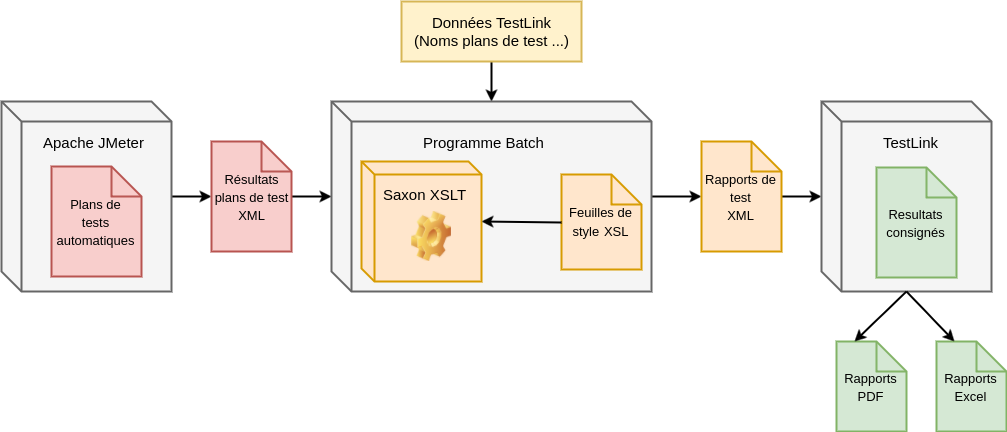
\includegraphics[scale=0.5]{images/travailNeuflizeOBC/testsFonc/testsProcedure.png}
	\centering
	\caption{Procédure de test finale}
	\label{testsProcedure}
\end{figure}

	Lors d'une livraison, une ressource pouvait parfois être occupé jusqu'à une demi-journée rien que pour exécuter l'ensemble des tests et consigner leur résultats, pour les raisons que nous avions évoquées partie \ref{testsFonc_03}. Avec cette nouvelle procédure, la génération des documents à destination du client prenait environ \textbf{10 minutes}, le plus long étant d'attendre la fin de l'exécution des tests automatiques. Ceci représente un gain de temps considérable pour l'équipe et permet d'obtenir des rapports conformes avec les besoins et attentes du client. De plus, cela a permis de soulager les développeurs d'un bon nombre de tâches répétitives et peu intéressantes d'un point de vue technique bien qu'essentielles dans le processus de satisfaction du client, dégageant ainsi du temps supplémentaire dans les sprints pour accomplir les objectifs fixés. \\
	
	Cependant, malgré les bénéfices apportés, certains points restent perfectibles. En effet, l'application web TestLink n'est pas actuellement hébergée sur un serveur dédié. Le projet touchant à sa fin, celui-ci sera repris par une équipe de maintenance qui aura besoin d'accéder à tous les outils et qui devra consigner les résultats de ses tests quotidiens c'est pourquoi il aurait été recommandé de pouvoir procéder à l'installation de TestLink sur un serveur dédié. 
	
	De plus, il aurait pu être intéressant de pousser l'automatisation des tâches à son maximum en ayant recours à Jenkins. En effet, il s'agit d'un outil d'intégration continue permettant d'automatiser différentes procédures. J'ai appris par la suite qu'un Jenkins aurait dû être mis en place au début du projet mais que cela n'avait pas été effectué faute de temps, il est prévu qu'un architecte se charge de cette installation. JMeter et TestLink sont tous deux compatibles avce cet outil tout comme les programmes Batch, il serait ainsi possible par la suite de programmer l'exécution des tests et la création des rapports de manière entièrement automatique à un intervalle de temps souhaité.
	\label{testsFonc_05}
	
\subsection{Aller plus loin : Tests de charge}
		L'équipe avait émis le besoin de mettre en place des tests de charge, JMeter étant installé et y étant formé j'ai pris en charge la réalisation de ces tests. Ces derniers consistent à mesurer le temps de réponse d'un système lorsque celui-ci est soumis à des conditions particulières afin de vérifier s'il est capable de soutenir le traffic attendu. Les conditions regroupent différents paramètres comme le temps de réponse, le volume du traffic, le nombre de requêtes effectuées en parallèle, la configuration du matériel ou encore la stabilité des serveurs. Afin de réaliser de tels tests, il faut dans un premier temps configurer l'environnement sur lequel ils seront exécutés. Dans notre cas, nous avions à notre disposition un environnement de pré-production (RGB) dont les caractéristiques étaient identiques à celles de la production, ce qui était approprié pour réaliser ce genre de tests. De plus, nous avions aussi l'environnement HOMO3 avec des capacités inférieures, idéal pour exécuter les tests dans des conditions un peu plus extrêmes dans le but mesurer la robustesse des APIs. \\
	
	Après cela, j'ai pris soin de définir différents scénarios de tests dont l'objectif étaient de simuler l'activité utilisateur afin de se rapprocher le plus possible des cas d'utilisation réels. Par exemple, un des scénario classique pourrait décrire la procédure suivie pour effectuer une transaction bancaire d'un compte vers un autre. Pour cela, l'utilisateur pourrait se connecter à l'application mobile puis initier sa transaction en choisissant des comptes débiteur et créditeur et il enfin il la signerait numériquement. De plus, celui-ci pourrait d'abord consulter ses comptes avant de prendre la décision de réaliser cette transaction. Les scénarios sont représentés par des diagrammes de cas d'utilisation comme celui présent sur la figure \ref{scenarioTest}, décrivant la réalisation d'une transaction. \\

	On peut ainsi remarquer rapidement les différents services (listés en annexe \ref{a2}) qui seront appelés lors de l'exécution de ce scénario :
	\begin{itemize}
		\item VKB pour générer le clavier virtuel permettant l'authentification et la signature de la transaction
		\item tokenInfo pour générer le token d'authentification
		\item newTransfer pour initier la transaction
		\item accountToDebit pour sélectionner le compte débiteur
		\item addressBook pour sélectionner le compte créditeur
		\item signByVKB pour signer la transaction
		\item clientList pour lister tous les comptes
		\item accountOverview pour consulter un compte particulier \\
	\end{itemize}
	
	Une fois les services identifiés, il ne restait plus qu'à construire le plan de test JMeter permettant de réaliser le scénario. Pour cela, j'ai réemployé la structure mise en place précédemment pour les tests fonctionnels. Cependant, j'ai supprimé l'ensemble des assertions puisque ces dernières peuvent influer sur les temps de réponse calculés par JMeter et n'ont pas d'intérêt dans un test de charge. Il ne restait donc qu'à modifier les scripts Beanshell déjà écrits pour les adapter à la situation. La principale différence réside dans la configuration du moteur d'utilisateur. En effet, sur les tests fonctionnels j'avais placé un tel moteur à la racine des plans afin qu'il englobe tous les composants. Ainsi, pour les tests de charges il suffisait de modifier les paramètres du moteur à savoir le nombre de thread, d'itération et le temps de montée en charge pour adapter les conditions d'exécution des scénarios sans avoir à modifier la structure des plans.
	
	Ces tests de charges ont par la suite été exécutés dans différentes conditions ce qui a permis de déceler certaines anomalies. \hl{TODO : exemple du probleme voir abdel}
	\label{testsFonc_06}